\documentclass[10pt]{article}

\usepackage[T1]{fontenc}
\usepackage{lmodern}
\usepackage{microtype}
\usepackage[margin=0.92in]{geometry}
\usepackage{amsmath,amssymb,amsthm,mathtools}
\usepackage{booktabs,tabularx,array}
\usepackage{enumitem}
\usepackage[dvipsnames]{xcolor}
\usepackage{tikz}
\usetikzlibrary{arrows.meta,positioning,calc,fit,shapes.geometric}
\usepackage{natbib}
\usepackage[colorlinks=true,linkcolor=MidnightBlue,citecolor=BrickRed,
  urlcolor=MidnightBlue]{hyperref}
\usepackage[nameinlink,noabbrev]{cleveref}
\usepackage{fancyhdr}
\usepackage{caption}

\definecolor{AuditBlue}{HTML}{173B57}
\definecolor{AuditTeal}{HTML}{087E8B}
\definecolor{AuditGold}{HTML}{B57A17}
\definecolor{AuditGray}{HTML}{F1F4F6}
\definecolor{AuditRed}{HTML}{8D2E2E}
\definecolor{AuditGreen}{HTML}{356859}

\newtheorem{theorem}{Theorem}[section]
\newtheorem{proposition}[theorem]{Proposition}
\newtheorem{corollary}[theorem]{Corollary}
\newtheorem{lemma}[theorem]{Lemma}
\theoremstyle{definition}
\newtheorem{definition}[theorem]{Definition}
\newtheorem{example}[theorem]{Example}
\theoremstyle{remark}
\newtheorem{remark}[theorem]{Remark}

\newcommand{\R}{\mathbb{R}}
\newcommand{\MMD}{\operatorname{MMD}}
\newcommand{\diam}{\operatorname{diam}}
\newcommand{\dir}{\operatorname{dir}}
\newcommand{\id}{\mathrm{id}}
\newcommand{\eps}{\varepsilon}
\newcommand{\cH}{\mathcal{H}}
\newcommand{\cP}{\mathcal{P}}
\newcommand{\cZ}{\mathcal{Z}}
\newcommand{\cX}{\mathcal{X}}
\newcommand{\EE}{\mathbb{E}}
\newcommand{\PP}{\mathbb{P}}

\setlist{itemsep=0.22em,topsep=0.35em}
\setlength{\parskip}{0.22em}
\setlength{\parindent}{1.15em}
\setlength{\emergencystretch}{3em}
\captionsetup{font=small,labelfont=bf}

\pagestyle{fancy}
\fancyhf{}
\fancyhead[L]{\footnotesize Permutation-cell auditing}
\fancyhead[R]{\footnotesize Anonymous research manuscript}
\fancyfoot[C]{\thepage}
\renewcommand{\headrulewidth}{0.3pt}

\title{\vspace{-1.6em}
{\color{AuditBlue}\bfseries Permutation-Cell Auditing}\\[0.3em]
\large Target-free falsification of all-order retrain equivalence\\
in sequential machine unlearning}
\author{Anonymous research manuscript}
\date{28 July 2026}

\begin{document}
\maketitle

\begin{abstract}
Sequential machine-unlearning services may process the same fixed deletion set
in different orders while claiming that every terminal model approximates one
common retraining result. Full retraining is often too costly to serve merely
as an audit oracle. We formulate and solve a narrower, one-sided problem:
when can deletion permutations themselves falsify a universal
retrain-equivalence tolerance?

We treat two orders as the boundary paths of a noncommutative comparative
statics (NCS) relation cell. For observed route outputs \(Y\) in any metric
space, their Chebyshev radius is the greatest population lower bound on
worst-route error obtainable from \(Y\) when the common target is otherwise
unconstrained; half the diameter is an always-valid weaker bound. Consequently,
an endpoint gap above \(2\eps\) rejects the claim that both routes are within
\(\eps\) of one target, without computing that target. Agreement cannot
certify deletion: all routes can coincide arbitrarily far from retraining.

For random outputs we give a simultaneous, finite-sample MMD margin rule with
family-wise error control. A Boolean-cube formulation identifies contextual
exchange cells, and a trusted affine promise reduces each cell to finitely many
basis probes. For a fixed-preconditioner relinearized ridge-deletion protocol,
we derive the exact cell defect, its global commutation criterion, quadratic
response order, and target-free retained-objective lower bound.

A reproducible 442-sample ridge case study checks all 97,461 deletion pairs,
executes all six orders of a three-request set, and supplies a powered
synthetic stochastic illustration. The artifact verifies the derived cell and
case-study formulas and uses exact retraining only afterward as a validation
oracle. The contribution is an
unlearning-specific synthesis and audit method, not a new Chebyshev, kernel,
commutator, or metamorphic-testing theorem.
\end{abstract}

\noindent\textbf{Keywords.}
machine unlearning; oracle-free auditing; path dependence; metamorphic testing;
Chebyshev radius; maximum mean discrepancy; noncommutative comparative statics.

\vspace{0.6em}
\begin{center}
\begin{minipage}{0.94\textwidth}
\colorbox{AuditGray}{%
\parbox{0.96\textwidth}{\small
\textbf{Claim boundary.}
PC-Audit is a sound, incomplete \emph{rejection} certificate for claims with one
common reset target or law. It does not certify that data were forgotten.
``Sharp'' refers only to a fixed observed population output set, with no
information about the target beyond membership in the declared metric space.
Finite-sample bounds are conservative, and unobserved orders remain
uncontrolled.}}
\end{minipage}
\end{center}

\section{Introduction}

Machine unlearning asks a trained system to remove the influence of selected
records more cheaply than full retraining
\citep{cao2015,ginart2019,bourtoule2021}. Strong formulations compare the
updated model or its law with the result of training on the retained data
\citep{guo2020,neel2021}. Approximate methods, however, are stateful numerical
protocols. Residuals are recomputed, optimizer state is carried forward,
preconditioners become stale, and stopping rules can depend on the path.
Deleting \(i\) and then \(j\) may therefore differ from deleting \(j\) and then
\(i\), even though the retained dataset is identical.

Order dependence is not itself new. Sequential deletion guarantees and
adaptive request streams are established topics
\citep{neel2021,gupta2021}; recent work directly studies forget-sample order in
gradient-ascent unlearning \citep{kumar2026}; and training-stage history can
obstruct path-oblivious retrain equivalence \citep{yu2025}. The question here is
more operational:

\begin{quote}
\emph{Can route disagreement alone prove that a universal all-order
retrain-equivalence tolerance is false, without constructing a retrained
reference?}
\end{quote}

The elementary triangle inequality suggests a pairwise answer, but turning it
into a useful audit requires several non-elementary choices: the quantifiers of
the claim, the sharp multi-route bound, stochastic-law semantics, a
level-controlled margin test, route failures, contextual rather than stateless
updates, finite auditability, numerical lower-bound safety, and an explicit
no-go boundary. We assemble these pieces as \emph{permutation-cell auditing}
(PC-Audit), an application of NCS to machine unlearning.

\paragraph{Contributions.}

\begin{enumerate}
  \item We identify the Chebyshev radius of a fixed observed route family as
  the sharp target-free population lower bound on its worst error to any
  otherwise unconstrained common reset target.
  \item We give a simultaneous bounded-kernel MMD lower confidence rule that
  rejects a common-target tolerance with controlled family-wise error.
  \item We present fixed deletion requests as a Boolean cube of contextual
  exchange cells and prove a complete finite test on a reachable affine hull
  under a trusted affine-map promise.
  \item We solve one concrete protocol exactly: fixed-preconditioner,
  relinearized ridge deletion. Its cell defect has a closed form, exact
  quadratic amplitude scaling, and a target-free retained-objective
  certificate.
  \item We provide a fully reproducible deterministic and stochastic case
  study, plus a no-go theorem showing why route agreement cannot positively
  certify unlearning.
\end{enumerate}

\paragraph{Recognizable review communities.}
The paper sits at the intersection of machine unlearning and auditing,
nonparametric kernel testing, numerical optimization, and metamorphic software
testing. Each mathematical ingredient is standard enough to admit conventional
review; the candidate novelty is the scoped synthesis and application.

\section{Related work and positioning}

\paragraph{Unlearning guarantees and approximations.}
Certified removal, deletion algorithms for convex models, SISA training, and
approximate linear-model deletion establish retraining-based or
distribution-based reference semantics
\citep{guo2020,neel2021,bourtoule2021,izzo2021}. Influence functions motivate
many local approximations \citep{koh2017}. PC-Audit does not propose a faster
unlearning update. It treats an existing update implementation as a response
protocol and tests a necessary consequence of a common-target claim.

\paragraph{Sequential and path-dependent unlearning.}
\citet{gupta2021} study adaptive deletion sequences.
\citet{kumar2026} directly show that different orderings of the same forget
samples can produce different outcomes in gradient-ascent unlearning.
\citet{yu2025} study dependence on earlier training-stage order. These works
preclude any claim that deletion-order sensitivity or local commutators are
new. Our fixed checkpoint and fixed deletion set instead support a
target-independent \emph{lower bound} against every common reset target.

\paragraph{Auditing and oracle limits.}
\citet{thudi2022} show why output or parameter proximity alone cannot prove
that data were absent from a training trajectory. Current work develops
retraining-free verification models \citep{ye2026}, representation-level
diagnostics \citep{cosma2026}, and validated selective screens while emphasizing
limits of oracle-free certification \citep{yang2026}. PC-Audit is deliberately
weaker: rejection is logically sound for a precisely declared target
tolerance, while non-rejection is inconclusive.

\paragraph{Metamorphic and kernel testing.}
Metamorphic testing evaluates relations among executions when a direct oracle
is unavailable \citep{segura2016}. PC-Audit is an unlearning-specific
metamorphic relation equipped with a metric target-error interpretation.
MMD and kernel two-sample testing are established
\citep{gretton2012}; current work includes equivalence margins
\citep{liu2026} and machine-unlearning-oriented divergence tests
\citep{ribero2026}. We do not introduce a new kernel test. We use a simple
simultaneous MMD lower confidence bound as input to the NCS geometric
conversion.

\section{Audit semantics}

Fix a finite, non-adaptively selected deletion set \(A\), a family
\(\Pi_A\) of permitted orders, and a starting checkpoint. Every
\(\pi\in\Pi_A\) has the same retained dataset \(D\setminus A\), so the routes
are externally equivalent. Their internal carried states may differ.

Let \((X,d)\) be the declared comparison space. Its points can be model
parameters, prediction vectors on a fixed probe set, functions modulo a gauge,
or probability laws. A successful route \(\pi\) returns \(y_\pi\in X\).
A chosen reset semantics supplies one common target \(t_A\in X\): for example,
the output of a deterministic canonical trainer on \(D\setminus A\), or the
law of a randomized canonical trainer.

\begin{definition}[Uniform all-order target claim]
\label{def:uniform}
The response protocol satisfies a uniform \(\eps\)-target claim on
\(\Pi_A\) if every route is defined and
\[
  d(y_\pi,t_A)\le \eps
  \qquad\text{for every }\pi\in\Pi_A.
\]
\end{definition}

Warm starts, cached state, stopping rules, and seed coupling belong to the
response protocol. They are not silently equated with reset retraining.
Route-conditioned, seed-coupled, or set-valued targets require a different
claim and are outside \cref{def:uniform}.

\begin{figure}[t]
\centering
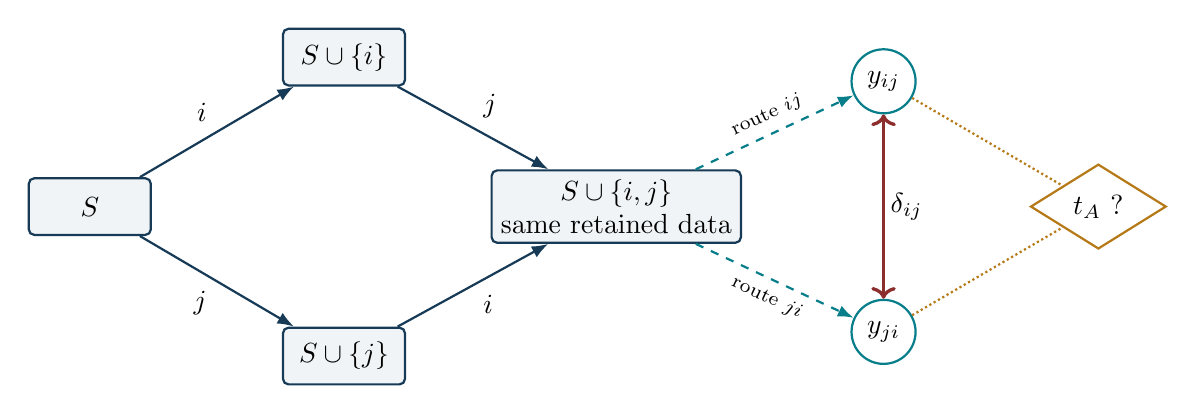
\begin{tikzpicture}[
  node distance=1.45cm and 2.4cm,
  state/.style={draw=AuditBlue,thick,rounded corners=2pt,
    fill=AuditGray,minimum width=1.55cm,minimum height=0.72cm,
    align=center},
  endpoint/.style={draw=AuditTeal,thick,circle,fill=white,
    minimum size=0.72cm},
  arr/.style={-{Latex[length=2.1mm]},thick,draw=AuditBlue}
]
\node[state] (S) {\(S\)};
\node[state,above right=1.15cm and 1.65cm of S] (Si) {\(S\cup\{i\}\)};
\node[state,below right=1.15cm and 1.65cm of S] (Sj) {\(S\cup\{j\}\)};
\node[state,right=4.3cm of S,minimum width=2.35cm] (Sij)
  {\(S\cup\{i,j\}\)\\same retained data};
\draw[arr] (S) -- node[above left] {\(i\)} (Si);
\draw[arr] (Si) -- node[above right] {\(j\)} (Sij);
\draw[arr] (S) -- node[below left] {\(j\)} (Sj);
\draw[arr] (Sj) -- node[below right] {\(i\)} (Sij);

\node[endpoint,above right=0.82cm and 1.5cm of Sij] (yij) {\(y_{ij}\)};
\node[endpoint,below right=0.82cm and 1.5cm of Sij] (yji) {\(y_{ji}\)};
\draw[-{Latex[length=2mm]},draw=AuditTeal,thick,dashed] (Sij) --
  node[above,sloped,font=\scriptsize] {route \(ij\)} (yij);
\draw[-{Latex[length=2mm]},draw=AuditTeal,thick,dashed] (Sij) --
  node[below,sloped,font=\scriptsize] {route \(ji\)} (yji);
\draw[<->,draw=AuditRed,very thick] (yij) --
  node[right,fill=white,inner sep=2pt] {\(\delta_{ij}\)} (yji);
\node[draw=AuditGold,thick,diamond,aspect=1.6,right=3.65cm of Sij]
  (target) {\(t_A\ ?\)};
\draw[densely dotted,draw=AuditGold,thick] (yij) -- (target);
\draw[densely dotted,draw=AuditGold,thick] (yji) -- (target);
\end{tikzpicture}
\caption{\textbf{Permutation cell.} The external square commutes because both
paths delete the same records. The response endpoints can disagree. Their
separation \(\delta_{ij}\) lower-bounds the worst distance to every unknown
common target by \(\delta_{ij}/2\).}
\label{fig:cell}
\end{figure}

\section{Sharp target-free geometry}

For a nonempty finite set \(Y=\{y_1,\ldots,y_m\}\subset X\), define
\[
  r_X(Y)=\inf_{z\in X}\max_a d(y_a,z),
  \qquad
  \diam(Y)=\max_{a,b}d(y_a,y_b).
\]
The infimum permits metric spaces in which no center is attained.

\begin{theorem}[Sharp output-only certificate]
\label{thm:radius}
For every common target \(t\in X\),
\[
  \max_a d(y_a,t)
  \ge r_X(Y)
  \ge \frac12\diam(Y).
  \tag{4.1}
\]
Moreover, \(r_X(Y)\) is the greatest lower bound guaranteed from the fixed
observed set \(Y\) alone when the target is otherwise unconstrained in \(X\).
Precisely, if \(B(Y)\) satisfies
\[
  \max_a d(y_a,t)\ge B(Y)
  \quad\text{for every }t\in X,
\]
then \(B(Y)\le r_X(Y)\).
\end{theorem}

\begin{proof}
Substituting \(z=t\) into the infimum gives the first inequality. For every
pair \(a,b\) and every \(z\),
\[
 d(y_a,y_b)\le d(y_a,z)+d(y_b,z)
 \le 2\max_c d(y_c,z).
\]
Maximize over pairs and infimize over \(z\).

For optimality, suppose \(B(Y)>r_X(Y)\). By the definition of an infimum,
some \(z\in X\) satisfies \(\max_a d(y_a,z)<B(Y)\), contradicting the proposed
guarantee at target \(t=z\).
\end{proof}

\begin{corollary}[Pair-cell rejection]
\label{cor:pair}
If \(d(y_\pi,y_\sigma)>2\eps\), no common target lies within \(\eps\) of both
routes. Hence the uniform \(\eps\)-target claim is false.
\end{corollary}

If independent information restricts \(t\) to a nonempty \(T\subseteq X\), the
stronger quantity is \(\inf_{z\in T}\max_a d(y_a,z)\). The sharpness claim in
\cref{thm:radius} assumes no such information. Likewise, an observed-route
radius does not control unobserved orders.

\subsection{Hilbert decomposition}

Let \(X\) be a real Hilbert space, with two outputs \(y_+\) and \(y_-\). Define
\[
  c=y_+-y_-,
  \qquad
  m=\frac{y_++y_-}{2}.
\]

\begin{proposition}[Two-route audit identity]
\label{prop:hilbert}
The unique two-point minimum-enclosing-ball center is \(m\), with radius
\(\|c\|/2\). For every target \(t\),
\[
 \frac{\|y_+-t\|^2+\|y_--t\|^2}{2}
 =
 \|m-t\|^2+\frac{\|c\|^2}{4}.
 \tag{4.2}
\]
\end{proposition}

\begin{proof}
Apply the parallelogram identity to
\(y_\pm-t=(m-t)\pm c/2\). The average of the two squared distances is at least
\(\|c\|^2/4\), while \(m\) attains equal distances \(\|c\|/2\).
\end{proof}

The midpoint removes the antisymmetric route component, but
\(\|m-t\|\) can remain arbitrarily large. This distinction is fundamental.

\begin{proposition}[Zero-defect no-go]
\label{prop:nogo}
No finite-valued function of route disagreement alone can uniformly
upper-bound reset-target error. For every \(M>0\), there is a protocol whose
routes all agree while their common output is distance \(M\) from the reset
target.
\end{proposition}

\begin{proof}
Take \(X=\R\), target \(t=0\), and every deletion map to be the constant map
\(x\mapsto M\). Every route has the same output and all relation-cell defects
vanish, while target error equals \(M\).
\end{proof}

Thus PC-Audit can falsify a target claim when its lower bound crosses the
declared tolerance. It cannot certify the claim when the bound is small.

\section{Stochastic route laws}

Let route \(\pi\) return a probability law \(P_\pi\) on \(\cZ\), and let the
selected reset law be \(Q_A\). Randomness semantics must match:

\begin{itemize}
  \item Cloning one trained checkpoint estimates conditional laws
  \(P_{\pi\mid W=w_0}\). It can audit only a matching conditional reset
  semantics.
  \item An end-to-end claim about the algorithmic marginal law requires
  independent reruns of both original training and unlearning.
\end{itemize}

A common-seed coupled difference is not by itself a difference between
marginal laws. Random route failure must either be represented by a
distinguished output symbol or audited with a separate failure-probability
tolerance. One crash rejects only an almost-sure availability claim.

\subsection{A simultaneous MMD margin certificate}

Let \(k\) be a characteristic positive-definite kernel with feature map
\(\phi:\cZ\to\cH_k\) and global diagonal bound
\[
  k(z,z)=\|\phi(z)\|_{\cH_k}^2\le K.
\]
For law \(P\), let \(\mu_P=\EE_P\phi(Z)\), so that
\(\MMD_k(P,Q)=\|\mu_P-\mu_Q\|_{\cH_k}\)
\citep{gretton2012}.

Suppose \(s\) routes are audited and route \(a\) supplies \(n_a\) independent
complete-route replicates \(Z_{a1},\ldots,Z_{an_a}\). Cross-route dependence,
including paired common random numbers, is allowed; within-route replicates
must be independent. Define
\[
 \widehat\mu_a=\frac1{n_a}\sum_{\ell=1}^{n_a}\phi(Z_{a\ell}),
\]
and, for \(0<\delta<1\),
\[
 e_a(\delta)
 =
 \sqrt{\frac K{n_a}}
 +
 \sqrt{\frac{2K\log(s/\delta)}{n_a}}.
 \tag{5.1}
\]

\begin{theorem}[Simultaneous MMD rejection margin]
\label{thm:mmd}
With probability at least \(1-\delta\), simultaneously for all routes,
\[
 \|\widehat\mu_a-\mu_a\|_{\cH_k}\le e_a.
 \tag{5.2}\label{eq:mmd-event}
\]
Consequently, every pair obeys
\[
 \MMD_k(P_a,P_b)
 \ge
 L_{ab}
 :=
 \left[
 \|\widehat\mu_a-\widehat\mu_b\|-e_a-e_b
 \right]_+.
 \tag{5.3}\label{eq:mmd-pair}
\]
If \(\widehat r\) is the minimum-enclosing-ball radius of the empirical mean
embeddings, then the population radius satisfies
\[
 r_{\cH_k}(\{\mu_a\})
 \ge
 L_{\mathrm{rad}}
 :=
 \left[\widehat r-\max_a e_a\right]_+.
 \tag{5.4}\label{eq:mmd-radius}
\]
Therefore either condition
\[
  \max_{a,b}L_{ab}>2\eps,
  \qquad\text{or}\qquad
  L_{\mathrm{rad}}>\eps
  \tag{5.5}\label{eq:mmd-reject}
\]
rejects, with family-wise error at most \(\delta\), the claim that every route
law lies within MMD distance \(\eps\) of one common reset law.
\end{theorem}

\begin{proof}
For one route, Jensen's inequality and independence give
\[
\EE\|\widehat\mu_a-\mu_a\|
\le
\sqrt{\EE\|\widehat\mu_a-\mu_a\|^2}
\le \sqrt{K/n_a}.
\]
Changing one replicate changes the empirical mean, and hence the norm of its
error, by at most \(2\sqrt K/n_a\). McDiarmid's bounded-difference inequality
\citep{mcdiarmid1989} yields
\[
\PP\left[
\|\widehat\mu_a-\mu_a\|>\sqrt{K/n_a}+t
\right]
\le
\exp\left(-\frac{n_at^2}{2K}\right).
\]
Set \(t=\sqrt{2K\log(s/\delta)/n_a}\) and union-bound over routes to prove
\eqref{eq:mmd-event}. The reverse triangle inequality gives
\eqref{eq:mmd-pair}.

On the event \eqref{eq:mmd-event}, corresponding empirical and population embeddings
are within \(\eta=\max_a e_a\). A finite-set minimum-enclosing-ball radius is
1-Lipschitz under such a Hausdorff perturbation: the same center enlarges a
ball by at most \(\eta\) in either direction. This proves
\eqref{eq:mmd-radius}. \Cref{thm:radius} completes the conversion to
\eqref{eq:mmd-reject}.
\end{proof}

\paragraph{Implementation safeguards.}
The statistic in \cref{thm:mmd} is the RKHS norm of empirical means, often
called biased MMD, not the possibly negative unbiased estimator of
\(\MMD^2\). Kernel, bandwidth, routes, tolerance, and transformations must be
fixed independently or handled by a valid selection procedure. A predeclared
finite kernel family can receive a multiplicity correction; continuous
data-adaptive optimization needs sample splitting or a uniform bound.
Approximate minimum-enclosing-ball software must return a certified lower
bound or subtract a proven optimization error before rejection.

\section{Deletion orders as a Boolean cube}

Let \(A=\{1,\ldots,q\}\). External vertices are subsets \(S\subseteq A\).
For \(i\notin S\), an edge \(S\to S\cup\{i\}\) processes request \(i\).
For \(i,j\notin S\), the contextual exchange square is
\[
\left(
S\xrightarrow{i}S\cup\{i\}\xrightarrow{j}S\cup\{i,j\}
\right)
\Rightarrow
\left(
S\xrightarrow{j}S\cup\{j\}\xrightarrow{i}S\cup\{i,j\}
\right).
\tag{6.1}
\]
There are \(\binom q2 2^{q-2}\) such squares for \(q\ge2\).

Let response edges be context-dependent partial maps
\[
  U_i^S:X_S\rightharpoonup X_{S\cup\{i\}}.
\]
Equal outputs are not enough when one route is undefined; equality of partial
maps requires both equal domains and equal values.

\begin{proposition}[Contextual-square completeness]
\label{prop:cube}
If the two composites on every contextual square have equal domains and equal
values, then every pair of monotone deletion paths with common endpoints
induces the same partial response map.
\end{proposition}

\begin{proof}
Any two permutations differ by adjacent transpositions. Each adjacent
transposition is one contextual square. Equality of partial maps is preserved
by composition, so a transposition chain transforms either path into the
other without changing the response map.
\end{proof}

For stateless total maps on one space, pairwise commutation is necessary and
sufficient for equality at every subset endpoint, or equivalently for all
request words up to permutation. It need not be necessary when only the one
full-set endpoint is checked: a noncancellative suffix can mask an earlier
defect. Approximate cells also require Lipschitz filling bounds, because a
suffix can amplify each local residual.

\subsection{Finite affine cell tests}

Suppose one contextual cell has a common affine domain and affine defect
\[
 \Omega(\theta)
 =
 U_j^{S\cup\{i\}}U_i^S(\theta)
 -
 U_i^{S\cup\{j\}}U_j^S(\theta).
\]
Let \(\theta_0,\ldots,\theta_r\) be an affine basis of an \(r\)-dimensional
reachable affine hull \(L\). Define linear maps \(V,W:\R^r\to\R^d\), with
\(V\) injective, by
\[
 Va=\sum_{k=1}^r a_k(\theta_k-\theta_0),
\quad
 Wa=\sum_{k=1}^r a_k
 \bigl(\Omega(\theta_k)-\Omega(\theta_0)\bigr).
\]
Then
\[
  \Omega(\theta_0+Va)=\Omega(\theta_0)+Wa.
  \tag{6.2}\label{eq:affine-reconstruction}
\]

\begin{proposition}[Affine-basis completeness]
\label{prop:affine}
The cell commutes on \(L\) if and only if its defect vanishes on one affine
basis of \(L\). On
\(\Delta=\operatorname{conv}\{\theta_0,\ldots,\theta_r\}\),
\[
 \sup_{\theta\in\Delta}\|\Omega(\theta)\|
 =
 \max_{0\le a\le r}\|\Omega(\theta_a)\|.
 \tag{6.3}\label{eq:simplex}
\]
\end{proposition}

\begin{proof}
An affine map is determined by its affine-basis values, proving
\eqref{eq:affine-reconstruction} and the first claim. For
\(\theta=\sum_a\lambda_a\theta_a\in\Delta\), convexity of the norm gives
\[
\|\Omega(\theta)\|
\le
\sum_a\lambda_a\|\Omega(\theta_a)\|
\le
\max_a\|\Omega(\theta_a)\|.
\]
The reverse inequality holds because the vertices belong to \(\Delta\).
\end{proof}

This finite test requires a trusted affine-map promise, a common valid domain
containing the hull, exact evaluations, and state-injection access. Basis
agreement cannot establish affineness. Noisy probes need a separate
conditioning-aware statistical analysis.

\section{Exact ridge relation-cell solution}

Consider the fixed-normalization ridge objective
\[
 F_D(\theta)
 =
 \frac12\sum_{k\in D}(x_k^\top\theta-y_k)^2
 +
 \frac\lambda2\|\theta\|^2,
 \qquad \lambda>0.
 \tag{7.1}
\]
Write
\[
 H=\lambda I+\sum_{k\in D}x_kx_k^\top,
 \quad
 b=\sum_{k\in D}y_kx_k,
 \quad
 \theta_D=H^{-1}b.
\]
Fix a symmetric positive-definite preconditioner \(P\). The
fixed-preconditioner relinearized request update is
\[
 U_i^\tau(\theta)
 =
 \theta+\tau P x_i(x_i^\top\theta-y_i),
 \qquad 0\le\tau\le1.
 \tag{7.2}\label{eq:update}
\]
It reevaluates request \(i\)'s residual at the carried state while retaining
the same preconditioner.

Let \(r_i(\theta)=x_i^\top\theta-y_i\) and
\(\alpha_{ij}=x_j^\top Px_i\). For a fixed start state, call \(p\) the
response order when a nonzero defect norm has leading scaling
\(C\tau^p+o(\tau^p)\) as \(\tau\downarrow0\), with \(C>0\).

\begin{theorem}[Exact ridge cell defect]
\label{thm:ridge}
For distinct requests \(i,j\),
\[
\boxed{
U_j^\tau U_i^\tau(\theta)-U_i^\tau U_j^\tau(\theta)
=
\tau^2\alpha_{ij}
\left[
Px_jr_i(\theta)-Px_ir_j(\theta)
\right].
}
\tag{7.3}\label{eq:ridge-defect}
\]
For \(\tau\in(0,1]\), nonzero features, and positive-definite \(P\), the two
affine maps commute at every state if and only if either
\[
x_i^\top Px_j=0,
\tag{7.4}
\]
or there is a nonzero scalar \(c\) with
\[
(x_j,y_j)=c(x_i,y_i).
\tag{7.5}
\]
At \(\tau=0\), both maps are identities. At a start state independent of
\(\tau\), a nonzero coefficient in \eqref{eq:ridge-defect} gives exact NCS
response order two: the defect scales exactly as \(\tau^2\).
\end{theorem}

\begin{proof}
Because
\[
r_j(U_i^\tau\theta)
=r_j(\theta)+\tau x_j^\top Px_i\,r_i(\theta),
\]
direct substitution in the two composites leaves \eqref{eq:ridge-defect}. If
\(\alpha_{ij}=0\), the defect vanishes. Otherwise the affine bracket vanishes
for every \(\theta\) exactly when
\[
x_jx_i^\top-x_ix_j^\top=0,
\qquad
x_jy_i-x_iy_j=0,
\]
after multiplying by \(P^{-1}\). Nonzero real vectors satisfy the first
identity precisely when \(x_j=cx_i\); the second then gives \(y_j=cy_i\).
The converse and the quadratic scaling are immediate.
\end{proof}

\subsection{Target-free retained-objective certificate}

Write \(U_i=U_i^1\), define
\[
z_{ij}=U_jU_i(\theta_D),
\qquad
z_{ji}=U_iU_j(\theta_D),
\]
and let \(\theta_{-ij}\) be the exact ridge minimizer after deleting \(i,j\).
The retained Hessian is
\[
H_{-ij}=H-x_ix_i^\top-x_jx_j^\top\succeq\lambda I.
\]

\begin{corollary}
\label{cor:objective}
In every norm,
\[
\max\{\|z_{ij}-\theta_{-ij}\|,\|z_{ji}-\theta_{-ij}\|\}
\ge \frac12\|z_{ij}-z_{ji}\|.
\tag{7.6}\label{eq:parameter-bound}
\]
Moreover,
\[
\begin{aligned}
\max_\pi\{
F_{-ij}(z_\pi)-F_{-ij}(\theta_{-ij})
\}
&\ge
\frac18\|z_{ij}-z_{ji}\|_{H_{-ij}}^2\\
&\ge
\frac\lambda8\|z_{ij}-z_{ji}\|_2^2.
\end{aligned}
\tag{7.7}
\]
\end{corollary}

\begin{proof}
Equation \eqref{eq:parameter-bound} is \cref{thm:radius} for two points. Since
\[
F_{-ij}(z)-F_{-ij}(\theta_{-ij})
=\frac12\|z-\theta_{-ij}\|_{H_{-ij}}^2,
\]
apply \eqref{eq:parameter-bound} in the \(H_{-ij}\)-norm and use
\(H_{-ij}\succeq\lambda I\).
\end{proof}

For \(m=(z_{ij}+z_{ji})/2\), the exact objective decomposition is
\[
\frac12\sum_{\pi\in\{ij,ji\}}
\left[
F_{-ij}(z_\pi)-F_{-ij}(\theta_{-ij})
\right]
=
\frac12\|m-\theta_{-ij}\|_{H_{-ij}}^2
+
\frac18\|z_{ij}-z_{ji}\|_{H_{-ij}}^2.
\tag{7.8}
\]
The last term is the identifiable antisymmetric order contribution. The first
is target-dependent and can remain large after route symmetrization.

\paragraph{Exact reset comparator.}
For batch feature matrix \(X_A\) and label vector \(y_A\), standard
Sherman--Morrison--Woodbury algebra \citep{golub2013} gives
\[
\theta_{-A}
=
\theta_D
+
H^{-1}X_A
\left(I-X_A^\top H^{-1}X_A\right)^{-1}
\left(X_A^\top\theta_D-y_A\right),
\tag{7.9}
\]
when the retained Hessian is positive definite. This exact set-dependent
reset commutes. It is used below only as a post-audit validation oracle.
Likewise, freezing all residual vectors produces commuting translations that
can still be wrong, illustrating \cref{prop:nogo}.

\section{Solved case study}

\subsection{Design and reproducibility}

We use the 442-sample, ten-feature diabetes dataset bundled with scikit-learn
\citep{pedregosa2011}. The target is population standardized, and
\(\lambda=0.05\). The study is mathematical and non-clinical: it makes no
predictive or population-generalization claim.

The protocol uses \(P=H^{-1}\) in \eqref{eq:update}. We exhaustively screen all
\(\binom{442}{2}=97{,}461\) record pairs by the analytic cell formula and
direct composition. The screen selects a strong transparent witness before
stochastic samples are generated. It is exploratory, not an estimate of
deployed prevalence.

The artifact pins NumPy 2.5.1, SciPy 1.18.0, and scikit-learn 1.9.0; records
the dataset-array, script, and requirements SHA-256 digests; fixes seed
20260728; and resolves its output path from the script location. All formulas,
checks, and values below are generated by one inspectable script.

\subsection{Two-route deterministic witness}

The strongest Euclidean cell uses records 32 and 322. Across all 97,461
pairs, the maximum discrepancy between analytic and directly composed defects
is \(2.26\times10^{-15}\). For the selected pair,
\[
\|z_{32,322}-z_{322,32}\|_2=0.0272943461,
\]
and in the retained-Hessian norm,
\[
\|z_{32,322}-z_{322,32}\|_{H_{-32,-322}}
=0.0115529959.
\]
Without using the reset target, \cref{cor:objective} therefore gives
\[
\max_\pi
\|z_\pi-\theta_{-32,-322}\|_{H_{-32,-322}}
\ge 0.00577649793
\tag{8.1}
\]
and
\[
\max_\pi
\left[
F_{-32,-322}(z_\pi)-F_{-32,-322}(\theta_{-32,-322})
\right]
\ge 1.66839642\times10^{-5}.
\tag{8.2}
\]

Only after computing the target-free quantities does the script solve the
exact retained-data solution. The two actual
parameter errors are 0.0102969 and 0.0107386 in the retained-Hessian norm,
while the objective excesses are \(5.30130\times10^{-5}\) and
\(5.76588\times10^{-5}\). The Pythagorean decomposition is
\[
5.53359\times10^{-5}
=3.86520\times10^{-5}+1.66840\times10^{-5},
\]
to \(6.61\times10^{-19}\) absolute numerical error. Thus 30.15\% of mean
two-route objective excess is the exactly identifiable antisymmetric order
component.

\begin{table}[t]
\centering
\caption{\textbf{Target-free quantities versus post-audit validation.}
Target-free columns use only route outputs and declared metric information.
Deterministic rows use an exact target computed afterward; the stochastic row
uses the closed-form population route radius and defines no reset law.}
\label{tab:case}
\small
\begin{tabularx}{\textwidth}{@{}l>{\raggedright\arraybackslash}Xrr@{}}
\toprule
Audit & Quantity & Target-free bound & Post-audit validation\\
\midrule
Pair \(\{32,322\}\) &
Worst parameter error, retained-\(H\) norm &
0.00577650 & 0.01073861\\
Pair \(\{32,322\}\) &
Worst retained objective excess &
\(1.6684\times10^{-5}\) & \(5.7659\times10^{-5}\)\\
Triple \(\{32,322,141\}\) &
Worst parameter error, retained-\(H\) norm &
0.01110879 & 0.03006635\\
Stochastic pair &
Route-law MMD radius &
0.23853627 & population radius 0.30764560\\
\bottomrule
\end{tabularx}
\end{table}

\subsection{Six routes and affine reconstruction}

For deletion set \(\{32,322,141\}\), all six orders are executed from the same
checkpoint. Their retained-Hessian diameter is 0.0222175847, so half the
diameter gives the target-free lower bound 0.0111087924. Exhaustive
floating-point support enumeration returns a minimum-enclosing-ball radius
equal to this value within \(10^{-15}\); the actual worst target error,
computed only for validation, is 0.0300663494. The bound recovers 36.95\% of
that witness's worst error. The diameter-supporting orders are
\((322,32,141)\) and \((141,32,322)\).

Because the ridge protocol is affine, one base point and ten coordinate probes
reconstruct the full cell defect. The linear-part Frobenius error is
\(4.26\times10^{-14}\), and the constant-part Euclidean error is
\(1.39\times10^{-13}\). One thousand random simplex probes respect the vertex
bound \eqref{eq:simplex}. Sampling illustrates rather than proves that bound; the
proof is \cref{prop:affine}.

\subsection{Response order and stochastic illustration}

At amplitudes
\[
\tau\in\{1,1/2,1/4,1/8,1/16,1/32\},
\]
the Euclidean defects are
\[
\begin{array}{c|rrrrrr}
\tau & 1 & 1/2 & 1/4 & 1/8 & 1/16 & 1/32\\
\hline
\|c_\tau\|_2 &
2.7294\!\times\!10^{-2} &
6.8236\!\times\!10^{-3} &
1.7059\!\times\!10^{-3} &
4.2647\!\times\!10^{-4} &
1.0662\!\times\!10^{-4} &
2.6655\!\times\!10^{-5}
\end{array}
\]
and the fitted log--log slope is 1.9999999999997464.

For a deliberately powered stochastic illustration, we add fresh independent
isotropic Gaussian noise to each complete route in retained-Hessian
coordinates. Noise scale and Gaussian-RBF bandwidth are effect-calibrated from
the deterministic witness, then fixed before random-number generation. This
is not a prospective power study.

With 3,000 replicates per route, \(K=1\), \(\delta=0.05\), and declared
\(\eps=0.10\),
\[
\widehat{\MMD}=0.612769,
\qquad
e_a=0.0678483,
\qquad
L_{12}=0.477073.
\]
Because \(L_{12}>2\eps=0.20\), \cref{thm:mmd} rejects the common conditional
reset-law tolerance with family-wise error at most 0.05. Equivalently for two
routes, the radius lower bound 0.238536 exceeds \(\eps\). The Gaussian
closed-form MMD is 0.615291; its
agreement with the realized lower bound is a one-seed consistency check, not
an empirical coverage estimate. Coverage follows from \cref{thm:mmd}.

\section{Operational PC-Audit protocol}

\begin{center}
\begin{minipage}{0.94\textwidth}
\colorbox{AuditGray}{%
\parbox{0.96\textwidth}{\small
\textbf{PC-Audit.}
\begin{enumerate}[leftmargin=1.4em]
  \item Declare one common reset target or law, comparison metric, tolerance,
  route family, and randomness semantics.
  \item Fix a non-adaptive deletion set. Clone one checkpoint only for a
  deterministic or conditional-on-checkpoint audit; rerun original training
  for an end-to-end marginal-law audit.
  \item Execute externally equivalent deletion orders. A deterministic route
  failure rejects the all-order availability claim. In a stochastic audit,
  include failure in the output law or audit its probability separately.
  \item Deterministic case: compute a certified Chebyshev-radius lower bound,
  or use half the observed diameter. Reject only if it exceeds \(\eps\).
  \item Stochastic case: compute \eqref{eq:mmd-pair} and, when numerically safe,
  \eqref{eq:mmd-radius}. Reject only under \eqref{eq:mmd-reject}.
  \item Under a trusted affine promise and state-injection access, reconstruct
  tested cell defects from affine-basis probes. Full path consistency requires
  every relevant contextual square and its domain.
  \item If no rejection occurs, report \textbf{inconclusive}, never
  ``certified unlearned.''
\end{enumerate}}}
\end{minipage}
\end{center}

\paragraph{Complexity.}
Two selected orders require two route executions. A full stateless pair audit
uses \(\binom q2\) cells, whereas a context-dependent Boolean cube contains
\(\binom q2 2^{q-2}\) cells. The full family can therefore be exponentially
large. Audit design must choose whether to test a specified small route set,
a risk-ranked sample, or a structural promise such as statelessness.

\paragraph{Metric choice.}
Parameter distance can be distorted by representation symmetries. Prediction
vectors on a fixed probe set or output laws may better match operational
claims, but probe selection and kernel bandwidth then enter the audit
specification. MMD detects differences in the declared output law; it is not a
privacy or deletion semantic by itself.

\section{Limitations and falsification conditions}

\begin{enumerate}
  \item \textbf{One-sidedness is unavoidable from route geometry alone.}
  \Cref{prop:nogo} rules out positive certification.
  \item \textbf{A common target is essential.} Route-conditioned,
  seed-coupled, or set-valued reset semantics require different geometry.
  \item \textbf{Observed routes are the scope.} A sharp radius on sampled
  routes says nothing about unobserved permutations without structural
  assumptions.
  \item \textbf{Context can be exponential.} Pairwise stateless commutation
  does not replace contextual cube cells in a genuinely state-dependent
  system.
  \item \textbf{Numerical lower bounds must be safe.} An approximate
  enclosing-radius overestimate can be anti-conservative. The case study uses
  half the diameter as the operative bound and treats its floating-point MEB
  as a diagnostic.
  \item \textbf{The case study is not a production benchmark.} It proves that
  the method can extract a nontrivial target-free certificate in an inspectable
  problem. Deep-model operational validation remains future work.
\end{enumerate}

The candidate novelty would be falsified by prior work that already combines
same-deletion-set permutations, the sharp common-target radius conversion, a
level-controlled stochastic margin rule, and the explicit one-sided
unlearning semantics. The mapped literature contains each ingredient or
nearby audit objective separately, but we found no such combined construction.
This is a positioning result, not proof of priority.

\section{Discussion}

The practical gain is not that a triangle inequality is difficult. It is that
the NCS presentation exposes a cheap, target-free observable with a precise
meaning. A route gap is no longer only ``instability.'' It is a lower bound on
the failure of a universal common-target claim. The Boolean cube says which
executions are comparable; partial-map semantics preserve directional
failures; the Chebyshev radius solves the multi-route geometry; the stochastic
bound matches probabilistic claims; and the no-go theorem prevents consistency
from being marketed as forgetting.

The ridge witness shows an additional benefit of the field-level view. The
cell defect separates into overlap,
\(\alpha_{ij}=x_j^\top Px_i\), and residual-weighted directions. It predicts
exact quadratic response order, identifies global commutation conditions, and
converts directly to retained-objective debt. These are actionable diagnostics:
an operator can rank request pairs by predicted defect, distinguish
orthogonality from duplicate labeled records, and quantify an unavoidable
worst-route error before paying for reset retraining.

The broader research direction is to develop relation-cell libraries for
actual unlearning protocols, safe adaptive route selection, interval-verified
radius solvers, function-space metrics invariant to parameter gauge, and
context-covering designs with explicit power and cost.

\section{Conclusion}

Permutation-cell auditing solves a concrete oracle-free problem for sequential
machine unlearning. If externally equivalent deletion orders separate by more
than twice a declared tolerance, then for every proposed common reset target,
at least one route lies outside tolerance. The observed Chebyshev radius is the
sharp unrestricted
population form of that statement; a bounded-kernel MMD margin provides a
finite-sample stochastic version. Boolean-cube and affine structure specify
when finite cell tests control larger path families, and an exact ridge example
demonstrates nontrivial target-free parameter and objective certificates.

The conclusion is deliberately asymmetric: disagreement can prove failure;
agreement cannot prove forgetting. That limitation is not a weakness hidden by
the method. It is the central fact that makes the method auditable.

\section*{Artifact availability and research conduct}

The accompanying artifact contains the checkpoint proofs, adversarial reviews,
literature collision map, pinned environment, executable case study, JSON
results, source manuscript, and rendered PDF. No external individual was
contacted during the research or review process; the recorded reviews were
performed by independent internal adversarial agents.

\bibliographystyle{plainnat}
\bibliography{references}

\end{document}
